% !TEX root =  ../main.tex
\section{Problem Statement}
\label{sec:problem}

%In the following, we will analyze the class of vulnerabilities that arise from the
%lack of controls on messagge passing through Intents, and we will formalize the problem we want to solve.

In this section, we provide a running example and illustrate the problem we are exploring.

% \subsection{Android Communication System Overview}

% Android applications are formed by a set of logically separated components
% (Activities, Services, Broadcast Receivers) that can communicate with each other
% during execution. Communication among these components is carried out by the IPC
% service of the operating system through a message passing mechanism, based on
% \emph{intents}. Essentially, \emph{intents} are messages containing a data portion, an action portion
% that tells the receiving application how to process the data, a category, and an optional
% component portion, which designates the receiving component.

% Components belonging to the same application can always communicate among each other via intents.
% To be able to receive intents sent by external applications, a component must
% explicitly declare an \emph{intent-filter} in the application's manifest file.
% Intent-filters describe the structure of intents (data types, actions, etc) a component is
% willing to receive and process. The operating system uses these \emph{intent-filters} to
% identify the recipient component of an intent, if not explicitly stated.

% The ability to receive intents from external applications is an important design feature of Android.
% In this way, applications can delegate tasks and communicate.
% The intent passing mechanism represents an often trusted communication channel
% in Android. However, Android itself does not provide mechanisms for applications
% components to verify the origin of intents. In particular, the most vulnerable
% components are those that expose intent-filters in the manifest file, enabling any application
% to send messages to those components. 

% \subsection{Threat Model and Running Example}
\textbf{Threat Model}. In our threat model, an attacker first analyzes the manifest file to identify exposed components that can receive intent messages. An example of such a component is depicted in Listing \ref{lst:example}, where the \textit{onCreate} method (line 1) is called to start a component. Next, the attacker identifies statements inside those components whose execution may be subverted to the attacker' s advantage. These statements may include network operations, database operations, updates to GUI elements and so on, and their execution may be subverted by modifying their parameter values, e.g., URL-s where data are sent by network operations, database queries, and the text of GUI elements. One such statement, dealing with a network operation is the HttpPost object creation in line 19. If the attacker is able to modify the value of the \textit{url} variable to a domain under the attacker's control or the value of the \textit{httpPar} variable to a string containing a cross-site scripting attack, then the component can be used to leak data to the attacker's web site or to execute a cross-site scripting attack, respectively. Another statement that may be of interest to an attacker is the one on line 31, which sets the path of a file that is ultimately sent over the network. If the attacker is able to modify the value of the variable \textit{p} (for instance, by including ``..'' in the path to perform directory traversal) together with the variable \textit{url}, then the component can be used to send arbitrary files to a host under the attacker's control. 
%We note however, that lines 13-14 sanitize the value of the \textit{file} variable before it reaches line 32. 
In the rest of this paper, we call such statements targeted by an attacker \textit{sink} statements.

Under this threat model, the only way in which the attacker can try to modify the parameters of the sink statements is by sending a specially crafted intent to the component via a malicious application installed on the user's phone. Thus, if the component is exposed, the attacker can control the values that that component receives in input (e.g., lines 2-5).

This attack vector has been recognized in the past by researchers and developers alike~\cite{Lu:CHEX:2012,chin2011analyzing,AppIntent,IntentsForDevelopers}. Two recommended practices for limiting this type of attacks are to not expose components needlessly and to sanitize and validate the data in input to the components. However, as often happens in application development, secure coding practices are not always followed. In fact, as shown by two independent studies of the first practice, a large percentage of applications still exposes components needlessly~\cite{Epicc,chin2011analyzing}. In addition, as shown by other studies, there may exist execution paths from (exposed) source statements to sensitive sinks~\cite{Lu:CHEX:2012}, along which data may flow. However, the presence of a path does not necessarily imply that an attack is feasible. In particular, applications may perform several operations along that path, such as sanitizations and other business logic operations. 

% \renewcommand{\lstlistingname}{}
\begin{lstlisting}[caption={Source code of a vulnerable application},label={lst:example},numbers=left,xleftmargin=1cm,basicstyle=\ttfamily\scriptsize ]
void onCreate(Bundle savedInstance) {
 Intent intent=getIntent();
 String host = intent.getStringExtra("hostname");
 String user = intent.getStringExtra("username");
 String file = intent.getStringExtra("filename");
 String url="http://www.example.com";
 if (host.contains("example.com"))
   url = "http://" + host + "/";
 if (file.contains(".."))
   file = file.replace("..", "");
 String userId = getUserID(user);
 if (userId != -1)
   textView.setText(user_name);
 String b64File = toBase64(file);
 String httpPar = toHttpParams(b64File,user_id);
 . . .
 try {
   DefaultHttpClient httpC = new DefaultHttpClient();
   HttpPost post = new HttpPost(url+httPar);
   . . .
   httpC.execute(post);
 }
 catch(IOException e) {
   e.printStackTrace();
 }
}
String toBase64(String p) {
 if(p=null || p.equals(""))
   p = "/data/data/com.example/defaultFile.pdf";
 else
   p = "/data/data/com.example/public/" + p;
 byte[] bytes = InputStream.read(p);
 String b = Base64Encoder.toString(bytes);
 return b;
}
\end{lstlisting}
% \normalsize
% \caption{Source code for the vulnerable application\label{fig:example-code}}
% \end{subfigure}
% \vspace{0.15in}
% \caption{A vulnerable application and its implementing code.}

In our example, we delineate three different operations that deal with the input variables. The first operation is a sanitization (lines 7-8) of the variable $host$. This sanitization is not sufficient, since an attacker can use any host name that contains the ``example.com'' string, e.g., ``malicious.example.com'' or ``example.com.com''. The value of \textit{host} set by the attacker inside the intent therefore flows unmodified to the sink statement at line 19. The second operation is also a sanitization (lines 9-10), which removes eventual ``..'' substrings from the file name to prevent directory traversal attacks. This sanitized value is then used later in line 31, which also adds a predefined prefix to the path. Thus, even though an attacker may be able to control to a certain degree the value of the variable \textit{p} at the sink statement (line 32), he cannot use it to perform a directory traversal attack. The third operation (lines 11-13) checks that the \textit{user} exists and sets a GUI element to a default user name if it does not exist. After this point, the value of the variable \textit{user} is not used by the program anymore. 

As has been recognized by previous work, to detect this type of vulnerabilities, it is important to correctly identify paths that starting from the \textit{source} statements enable an attacker to influence the variable values at the \textit{sink} statements. However, the existence of a path does not imply that an attack is feasible. To precisely identify exploit opportunities and prevent them, the operations performed on the variable values along that path must also be considered. In fact, these operations may include  sanitizations (e.g., lines 9-10), and other business logic operations (e.g., lines 11-13) that, while allowing an attacker to influence the values at the sink statements, make exploits unfeasible. An approach that includes these path operations in its analysis is therefore needed to precisely identify exploit opportunities and prevent them. Such an approach must also provide a vulnerability proof under the form of malicious input to the component, in order to verify the vulnerability. In the rest of the paper, we present a method for automatically detecting such vulnerabilities and providing proofs for them. 

%Rigel: this may be fitted for later
%The constraints for this variable will look like:
%\lstset{numbers=left, basicstyle=\ttfamily\scriptsize, breaklines=true}
%\begin{lstlisting}
%$hostname.contains("example.com") ->
%   $url :=  "http://" + $hostname + "/"
%(not $hostname.contains("example.com")) ->
%   $url :=  "http://www.example.com/"
%\end{lstlisting}

%Since the second clause does not lead to a propagation of $hostname$ to the sink, the solver is
%able to generate an exploit satisfying the first constraint. The solution will be $example.com@$ where the ``$@$'' symbol stays for any string.

%\item \emph{Exhaustive sanitization}. This happens for the path parameter encountering one control (line $13$) and two manipulations at line $14$ and $32$. Whereas the check and the first manipulation can be easily passed by providing a non-null string and not containing any ``$..$'' sequence, this is not sufficient for an attack to succeed. Indeed the string preponed to the path parameter at line $32$, binds the path to the application public folder. This manipulation and the
%absence of the double dot sequences in the path variable successfully prevents an attacker access of the application private files.
%Here below are the constraints:
%\lstset{numbers=left, basicstyle=\ttfamily\scriptsize, breaklines=true}
%\begin{lstlisting}
%$filename.contains("..") ->
%   $filename.replace("..", ".")
%$filename.length > 0
%$filename := "/data/data/com.example/public/" + $filename;
%\end{lstlisting}
%In this case, in order to have a correct problem formulation, we need to consider the sink semantic.
%The correct formulation for the $InputStream.read$ sink includes one more constraint for the string
%to be free (i.e. without manipulation).


%\item \emph{Unreachable sink}. Parameter $username$ is not exploitable.
%For this example we need to assume that the function $getUserID$ (line $10$) returns the user id
%if a username is found in the local database, $-1$ otherwise.
%A solution to this constraint can not be found since it would assume a complete knowledge of the
%dynamic environment, represented in this case by the local database.
%
%Also in this case the solver will be unable to find a solution for the constraint, since it will
%lack of bounds to produce a result. This vulnerability will be indeed reported correctly as unfeasible
%by our analyzer.


%\label{sec:running-example}
\todo{Edited code}
% \begin{figure*}[t]
% \centering
 %  \begin{subfigure}[b]{3.5in}
	% 	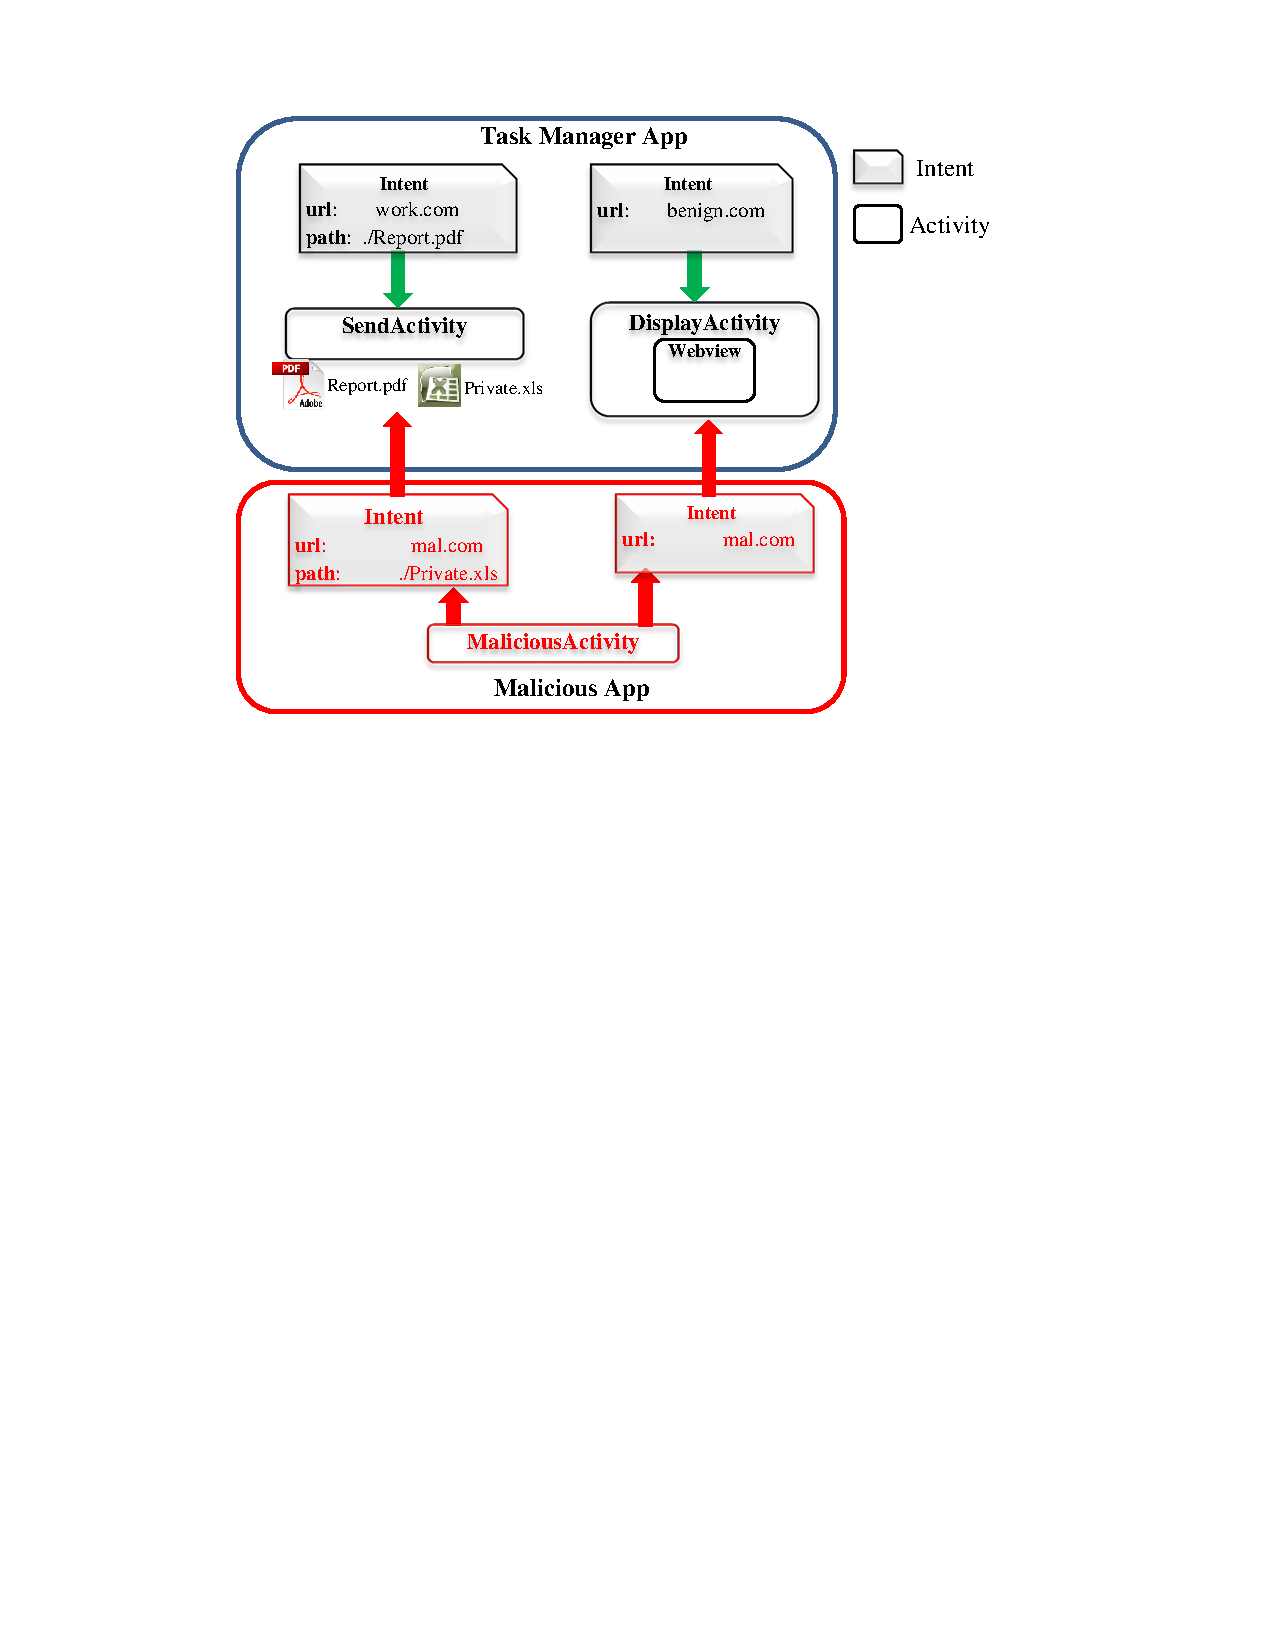
\includegraphics[width=3.3in]{./images/example.pdf}
 %                \caption{An example of vulnerable application.\label{fig:example-dia}}
	% \end{subfigure}%
        ~~~~~~~~~~~~ %add desired spacing between images, e. g. ~, \quad, \qquad, \hfill etc.
          %(or a blank line to force the subfigure onto a new line)
% \begin{subfigure}[b]{3in}
% \end{figure*}














%=========================
%TEXT FROM PREVIOUS VERSION


%We call this vector of attacks \emph{intent-spoofing attacks}. As illustrated by the examples,
%this attack may be performed by crafting intents that match the intent-filters declared by
%legitimate application components activities but contain data inserted by an attacker. The structure of such intents
%may be easily discovered by either looking at the manifest file of an application or by studying
%the (decompiled) code of the target application.

% \subsection{High Level Approach Overview}
% Our goal in this paper is to automatically identify opportunities for intent-spoofing attacks by modeling the relation between data input via intents and data output by an application component.

% Given an apk file, we first, we collect the entry points where malicious data may be received via intents and the sensitive operations
% where the results produced by a component are sent in output.
% %In this regard, we consider a wide range of operations executed
% %by framework method calls that includes output network operations, operations that execute SQL queries, and operations that update or create GUI elements. The range however may be extended to other output operations, such as those related to writing to the local file system.
% %For instance, lines 11 and 13 in the code example are identified as \emph{sources}, since
% %they are used to extract the data from the received intent.
% Next, using interprocedural data-flow analysis and taint analysis, we trace and collect the statements that process the intent data from the entry points to the sensitive operations that produce the output, thus obtaining several computation paths from the entry point to the output points. A detailed description of our analyzer is provided in Section \ref{staticAnalyzer}.
% %For instance, line 21 in the code example, which sends
% %data over the network is a \emph{sensitive sink} and the path comprising the statements at lines (11, 13, 14, 15, 18, 19, 21)
% %is a path where intent data flow from the sources to the sink.

% After the possible computation paths are identified, we need to prove that those paths are feasible at run time and that they can indeed be used by an attacker to subvert the intended behavior of the program.
% In fact, the existence of a path does not necessarily imply that the path can be useful for an attack.
% If, for instance, an activity validates the data along a path, then that path is not vulnerable. Our tool considers the different
% types of statements present in a path and automatically generates an intent with data that can be used to carry out an attack.
% This last step is described in more detail in Section \ref{sec:ExploitGenerator}.

%There are to ways to do this: fuzzying, app analysis.
%We are looking at analysis.
%High Level Overview:
%Goal: given the apk file, we want to
%see this app. During its execution it receives intent messages of two kinds.
%We want to see if an adversary can send from an untrusted component the integrity
%of an application. To understand, we must see how messages are received and processed
%by android. they are sent by a sender, received by a target,
%and processed in-application. Since the sender is untrusted we want ot
%identify in the app, the source. But this is not enough. Adversary needs to
%get to the sensitive sinks. In between we need to see how the message payload
%is processed.
%So our goal: Is a path possible between source and sink. This is data flow analysis:
%described in Section 3.2. Just identifying a path is not enough, we also need to prove that it
%is vulnerable. So we need to see what actions are being taken on that path.
%We need to


%
% Nonetheless, this type of open channel is present in many
%applications. Furthermore, due to the mistaken assumption that all intents sent at a target activity originate inside legitimate activities, the received data are not validated or sanitized before being passed to the rest of the application.
%Unfortunately, the Android IPC system does not provide mechanisms that can help verify the origin of an intent.


%\begin{itemize}
%  \item \textbf{Server attacks}: these attacks are similar to CSRF
%  attacks and to permission redelegation attacks identified in~\cite{felt2011permission}.
%  A malicious application sends to a component an Intent message that matches
%  the intent filters exposed by that component. Trusting that the intent originates
%  from a legitimate activity, the component does not validate the intent's data,
%  processes them according to some semantics and sends a request to a remote server.
%  Similarly to CSRF attacks, the request will be created within the normal request context.
%  That is, the request may be augmented with additional information, e.g. user-session
%  identifiers. The attack described in the example belongs to this category. %The attack, in this case, can be crafted
%%transparently with respect to client/server full-stack architecture, but taking
%%in consideration only Intent payload parts included in the request.
%
%%  As example, we can think of a bank application in which the mobile wire
%%transfer is implemented by the help of two activities: in the first activity,
%%the user is requested to insert the payee account and the amount. When the users
%%confirms, the information is sent as Intent payload to a second activity which
%%commits the transaction on the bank server. An attacker, by crafting the
%%exchanged Intent, could induce the second activity to perform a transfer on
%%behalf of the user to an arbitrary beneficiary.
%
%  \item \textbf{Storage attacks}: if intent data are used to
%build a query unsafely, even in case of Intent messages
%exchange we can have classical SQL Injection attacks \footnote{what does 'even in case of
%Intent messages exchange mean?}. Besides SQL Injection
%attacks, there can be identified other potentially dangerous attacks where the
%Intent receiver logic includes local storage operations and it is exposed via Intent
%receivers.
%%  These attack target logical vulnerabilities in application design, i.e.
%%situations in which local storage modifications are delegated to some particular
%%component which is queried via Intents.
%
% For instance, let's take into consideration another two activities example that implements a
%PIN change in an application where this code is used to guarantee
%application access. In the first activity a new PIN is collected from
%the user, then, in the second activity the old PIN is replaced with the new one
%by a database query. Similarly to the previous case, an attacker could arbitrary
%change the PIN by crafting an Intent with a different PIN, denying further application
%access to the user.
%
%  \item \textbf{Phishing attacks}: often intents are used to send data that
%  are displayed by the target Activity to the user.
%  An attacker could craft an intent containing fake data and send this intent to
%  the target Activity, thus prompting the fake data to the user.
%  To make this attack more effective, an attack may be designed to launch
%a series of Activities that exactly reconstruct the Activity sequence of
%the application, modifying the data displayed to the user at points of the
%attacker's choosing \footnote{we spoke about this type of attack before but the description
%must be more convincing. If we leave it at this rough level of detail it may sound
%unconvincing to the reader}.
%In this case, the deception could be very effective, since the
%user may think at herself as the author of the sequence of actions that produced
%the prompted screen.
%
%  A particular and remarkable variation of this attack is feasible when the intent
%  contains a URL of a page to be loaded in a web view. The vulnerable component
% In this case the attack
%can be even more effective, because of the image and general visual context
%that can be recreated inside a web view \footnote{is it more effective because
%it is easier to craft a web page very nicely?}.
%\end{itemize}
%
%This attack channel has been recognized by
%Android developers and researchers alike \cite{chin2011analyzing,felt2011permission}.
%In addition, application developers are warned against exposing activities via \emph{intent-filters} on
%the official Android documentation web site. Nonetheless, this type of open channel is present in many
%applications. Furthermore, due to the mistaken assumption that all intents sent at a target activity originate inside legitimate activities, the received data are not validated or sanitized before being passed to the rest of the application.
%Unfortunately, the Android IPC system does not provide mechanisms that can help verify the origin of an intent.
%
%An important thing to note at this point is that just the presence of an open channel does not
%necessarily imply that sensitive operations will be carried out by sending a spoofed intent.
%In fact, an open channel is exploitable in meaningful ways only if the
%flow and use of intent data inside an activity leads to eventually sensitive
%operations such as sending files to email addresses.
%
%The problem that we deal with in this paper is to automatically find \emph{sensitive paths} from the
%points in which intents are received (\emph{sources}) to sensitive API operations (\emph{sinks}) inside an
%application component.
%We use a rather general definition of sensitive API operations, which includes network communication
%APIs, database APIs, and UI APIs. This problem is depicted in figure \ref{fig:paths}. Given an intent
%with a certain information payload, the problem is that of finding all the paths through the component
%that start at the payload extraction site and end in one of the sinks.
%
%
%\begin{figure}[h!]
%  \centering
%    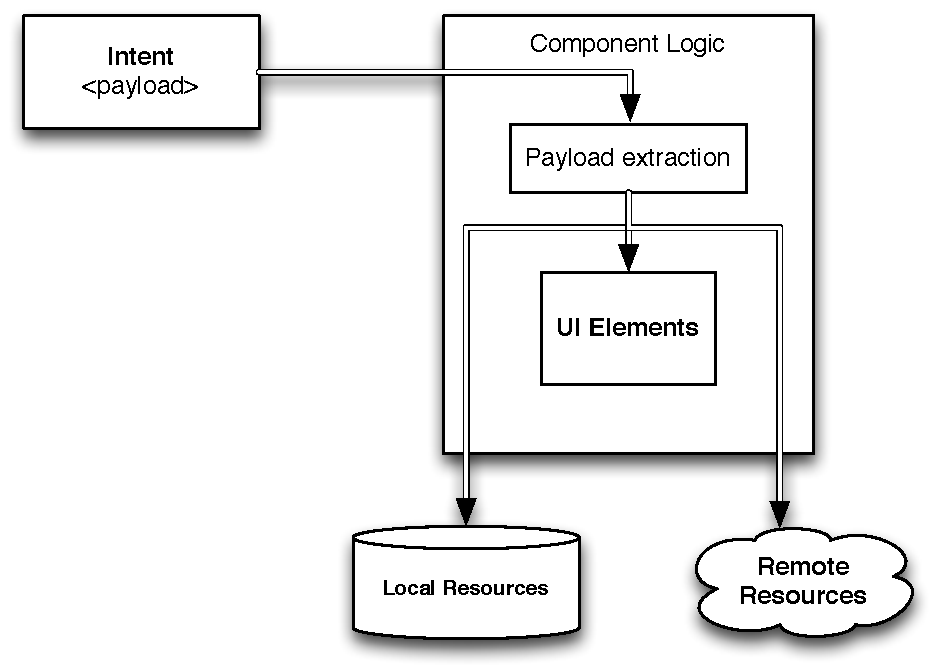
\includegraphics[width=0.5\textwidth]{images/paths.pdf}
%  \caption{Attack scenario \label{fig:paths}}
%\end{figure}
%
%Our tool discovers these sensitive paths through static analysis of an activity's code.
%To prove that the activity is exploitable along these paths, an additional step
%is needed. In fact, the existence of a path does not necessarily imply that run time
%execution of the activity will run along that path. Thus an additional problem we deal
%with this paper is that of finding such feasible paths.
%
%To this end, we design an analyzer that is able to track the path of intent data from
%sources corresponding to intent receivers to sinks corresponding
%to method calls and APIs used to send the data to the network, to databases,
%or to UI elements. Once such a path is identified, our tool automatically
%produces an intent example that can exploit that path.
